\documentclass{article}
\usepackage[utf8]{inputenc}
\usepackage{amsmath, amssymb}
\usepackage{graphicx}
\usepackage{wrapfig}
\usepackage{alltt}
\usepackage[margin=1in]{geometry}
\graphicspath{{./images/}}


\title{Correlation Between Key Stats and Challenge Rating in D\&D}
\author{William Jardee}
\date{March 2020}

\begin{document}
\maketitle

\par One on my personal hobbies is the table top game Dungeons \& Dragons. The general premise of the game is to play as a group of adventurers exploring a fantastical world and creating awesome, unique stories. As the story unfolds, the protagonists go up against various monsters. To help keep these encounters fair and engaging, the difficulty is calculated through simple algebra based on a stat called Challenge Rating. The purpose of this study is to find out how a couple select monster stat's affect the overall Challenge Rating of that monster. My general hypothesis is that AC, HP, and average ability score all play a strong relationship to the CR (Challenge Rating) of a monster. If we look at the co-variance matrix it will obviously be dominated by the HP since the average value will be much larger than the rest of the values. I expect to see a linear or quadratic curve to fit all three of the data sets to CR well.
\par The final data set used was one by RufflesDMAccount on Reddit (https://www.reddit.com/r/
UnearthedArcana/comments/8zvr6s/the\_great\_dd5e\_monster\_spreadsheet/). Initially the tests were done with a smaller set in a blog by Miroslav Zadravec (http://miroz.com.hr/random/ monsters.html), but moved over to the spreadsheet from the Reddit post because it provided a vast increase in data points. The data set came out to about 800 entries collected from Dungeons \& Dragons source books and generally accepted homemade creations.

%Covariance of AC,HP,Average ability score
\par First the data was loaded into Matlab and a quick co-variance test was ran on a matrix of AC, HP, and average ability score. Pulling the first principle component gave an eigen pair of 
$$\left( 9.07\times 10^{13}, \begin{bmatrix}0.0841\\0.9934\\0.0780\end{bmatrix}\right)$$
As to be expected the variance from the HP is massive compared to the other two of $1.85\times 10^8$ and $0.163$. The second largest impact, for the second largest principle component, was AC and then Average ability score.

%Testing each of the individual stats
\par At the end of the Matlab code a co-variance examination of the distribution of stats against the CR was run. I predicted that the three most important would be Strength, Constitution, and Wisdom. These predictions were drawn from knowledge of the game and a quick glance through the list. Below is the resulting principle matrix:
$$\begin{bmatrix}
-0.3516& 0.3477& 0.1911&-0.0968&-0.7189& 0.4390\\
 0.0247& 0.0382& 0.3727&-0.8823& 0.2727& 0.0794\\
 0.7195&-0.4696&-0.0367&-0.0991&-0.3687& 0.3386\\
 0.3324& 0.4599& 0.3253& 0.3441& 0.4211& 0.5259\\
 0.0621& 0.3327&-0.8450&-0.2795& 0.1160& 0.2825\\
-0.4937&-0.5787&-0.0582& 0.0767& 0.2865& 0.5745\\
\end{bmatrix}$$
The value of their respective eigenvalues are increasing right to left, so the first principle vector is in the 6th column, second principle vector in the 5th column, etc. To interpret this mess of values, the three most important abilities are Charisma, Strength, and Dexterity, in that order. However, since the eigenvalues are all pretty well distributed on the first principle component, which is the major axis, there is not one single stat that obviously dominates in importance.

%Least squares graphs 
\par Next, to analyze the least squares relationship between the challenge rating of monsters and the AC, HP, and average ability modifier. There is obviously not one perfect line for each relationship, as there are just too many points, so least squares is a logical process to develop a solution. If the sum of squares of errors is zero, then there was one line that fit all of the points. Initially a linear fit was applied to all three values and gave decent results, but, just from visual approximation, a quadratic solution looked better for the average ability modifier.
\begin{figure}
\begin{center}
    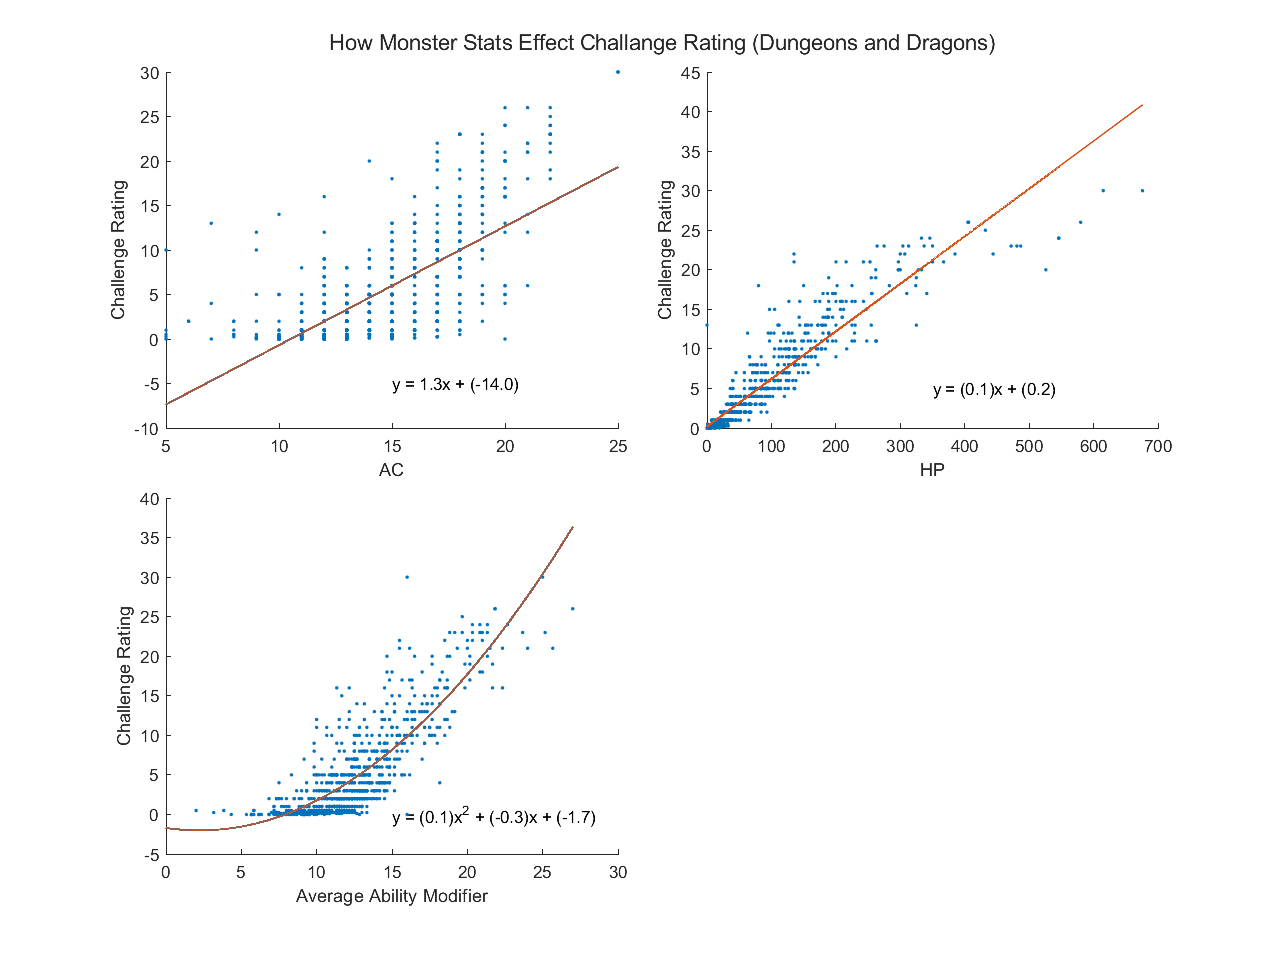
\includegraphics[width = \textwidth]{Graphs.png}
    \end{center}
    \caption{Data Sets with Least Squares Line Fits}
    \label{fig:my_label}
\end{figure}
Attempting to fit a logarithmic relationship failed because of the number of times there would be the natural log of zero while fitting for a solution. Investigating the issue online, it seemed that the solution was attempting the problem from a statistics approach of least squares. Seeing how this is outside of the scope of linear algebra based least squares, the best fit will be given as quadratic. For all three lines, calculating $(A^TA)^{-1}A^T$ did not return a singular matrix, so each has a unique solution to the least squares problem.
\par As it can be seen, these fits follow the general trend of the data, but are not overly good matches. Looking at the SSE of each least squares solution, the fit for AC gives $SSE\approx 15,308$, for HP $SSE\approx 4,345$ and for Ability Modifiers $SSE\approx 8,359$. A large part of error comes from how poor the fits are, but also from how many point there are. If the average difference was just 1.5, then $SSE \approx 1,800$, meaning a small variation still compounds quickly with this method. Curious if a better fit could be found by combining all three of these values into one equation, the least squares solution for all three data points were tested. The least squares solution turned out to:
$$(Chal) = 0.0206 + 0.3278(AC) + 2.9159(HP) + 0.3011(Abilities) + 4.7260(Abilities)^2$$
This solution atrociously fitted the data, giving $SSE \approx 1.27\times 10^{35}$. While the hypothesis assumed more variables would give a closer approximation, in reality it seems that the errors compounded to give an unusable relationship.
\par In conclusion, studying the effects that AC, HP, and ability modifiers, both average and individual, have on the challenge rating of popular monster in Dungeons \& Dragons, it seems many factors play a part in a complex relationship to form the challenge rating. The game is a complex array of components and dynamic pieces. Looking into the surprising outcome of the most important stat in considering challenge rating, Charisma, another hypothesis could be that stronger spells from the players challenge the Charisma of the monster. In the next couple months I plan to analyze the combination of monster challenge rating to player spells and a number of other variables in the game. To assess AC, HP, and Average Ability Score, there is an obvious relationship between each stat and a monster's challenge rating; however, the relationship is not fully clear from this analysis.
\newpage
\section{Madlab Code:}
\begin{alltt}
\input{code.txt}
\end{alltt}

\end{document}